\documentclass{article}

\usepackage{arxiv}

\usepackage[utf8]{inputenc} % allow utf-8 input
\usepackage[T1]{fontenc}    % use 8-bit T1 fonts
\usepackage{lmodern}        % https://github.com/rstudio/rticles/issues/343
\usepackage{hyperref}       % hyperlinks
\usepackage{url}            % simple URL typesetting
\usepackage{booktabs}       % professional-quality tables
\usepackage{amsfonts}       % blackboard math symbols
\usepackage{nicefrac}       % compact symbols for 1/2, etc.
\usepackage{microtype}      % microtypography
\usepackage{lipsum}
\usepackage{graphicx}

\title{Evolution, functional diversity, regime shifts, hysteresis, and
nonlinearity; ecosystem responses to environmental change.}

\author{
    Owen L Petchey
   \\
    Department of Evolutionary Biology and Environmental Studies \\
    University of Zurich \\
  Zurich 8057, Switzerland \\
  \texttt{\href{mailto:owen.petchey@ieu.uzh.ch}{\nolinkurl{owen.petchey@ieu.uzh.ch}}} \\
   \And
    Rainer Krug
   \\
    Department of Evolutionary Biology and Environmental Studies \\
    University of Zurich \\
  Zurich 8057, Switzerland \\
  \texttt{\href{mailto:rainer.krug@ieu.uzh.ch}{\nolinkurl{rainer.krug@ieu.uzh.ch}}} \\
   \And
    Any Others
   \\
    Department of Evolutionary Biology and Environmental Studies \\
    University of Zurich \\
  Zurich 8057, Switzerland \\
  \texttt{\href{mailto:any.others@ieu.uzh.ch}{\nolinkurl{any.others@ieu.uzh.ch}}} \\
   \And
    Marcel Suleiman
   \\
    Department of Evolutionary Biology and Environmental Studies \\
    University of Zurich \\
  Zurich 8057, Switzerland \\
  \texttt{\href{mailto:marcel.suleiman@ieu.uzh.ch}{\nolinkurl{marcel.suleiman@ieu.uzh.ch}}} \\
  }


% Pandoc citation processing
\newlength{\csllabelwidth}
\setlength{\csllabelwidth}{3em}
\newlength{\cslhangindent}
\setlength{\cslhangindent}{1.5em}
% for Pandoc 2.8 to 2.10.1
\newenvironment{cslreferences}%
  {}%
  {\par}
% For Pandoc 2.11+
\newenvironment{CSLReferences}[2] % #1 hanging-ident, #2 entry spacing
 {% don't indent paragraphs
  \setlength{\parindent}{0pt}
  % turn on hanging indent if param 1 is 1
  \ifodd #1 \everypar{\setlength{\hangindent}{\cslhangindent}}\ignorespaces\fi
  % set entry spacing
  \ifnum #2 > 0
  \setlength{\parskip}{#2\baselineskip}
  \fi
 }%
 {}
\usepackage{calc} % for calculating minipage widths
\newcommand{\CSLBlock}[1]{#1\hfill\break}
\newcommand{\CSLLeftMargin}[1]{\parbox[t]{\csllabelwidth}{#1}}
\newcommand{\CSLRightInline}[1]{\parbox[t]{\linewidth - \csllabelwidth}{#1}\break}
\newcommand{\CSLIndent}[1]{\hspace{\cslhangindent}#1}



\begin{document}
\maketitle

\def\tightlist{}


\begin{abstract}
To be completed
\end{abstract}

\keywords{
    Biodiversity
   \and
    Evolution
   \and
    Hysteresis
   \and
    Alternate stable states
   \and
    Environmental change
   \and
    Regime shift
   \and
    Threshold
   \and
    Ecosystem
   \and
    Cyanobacteria
   \and
    Sulfur bacteria
  }

\hypertarget{introduction}{%
\section{Introduction}\label{introduction}}

This report concerns how biodiversity influences the strength and nature
of ecosystem responses to environmental change (figure 1; panel(a) three
ovals, environment oval with arrow to ecosystem property oval, with
biodiversity oval pointing the arrow between environment and ecosystem
property; panel (b) shows linear response with different gradients,
large being with low diversity; panel (c) shows a linear and a
non-linear response starting and ending at the same place; panel (d)
shows a hysteretic response, with greater or less range of hysteresis).
Strong responses of ecosystems to environmental change imply high
\emph{sensitivity} and lack of resistance to environmental change, and
higher temporal variability in the face of varying environmental
conditions. Greater \emph{non-linearity} in ecosystem responses
increases the potential for surprises, such as when an ecosystem that
was resistant to an environmental change becomes unexpectedly sensitive
to further change. The presence and extent of \emph{hysteresis} in
ecosystem responses to environmental driver gradients concerns how
readily are ecosystem responses reversed when environmental change is
reversed.

In this context, a directly relevant aspect of biodiversity is variation
in functional traits, i.e.~the traits that determine organismal
responses to environmental conditions and that determine the effects of
organisms on their environment (citation). Variation in functional
traits is often termed ``functional diversity.'' There is a considerable
amount of theory predicting, and evidence supporting, that greater
functional diversity leads to lower temporal variability in ecosystem
states variables (such as total biomass) (citations) (Leary, Pennekamp).
The mechanism by which this occurs is that greater functional response
diversity causes a weaker relationship between an environmental driver
gradient and the ecosystem state (figure 1a/b), due to the functional
turnover along the environmental driver gradient that results from
variation in organisms' responses to the environmental driver gradient
(citation).

There is less theory about effects of functional diversity on the
linearity (figure 1c) and the hysteresis (figure 1d) of ecosystem
responses to environmental change. Dakos et al. (2019), in their article
\emph{Ecosystem tipping points in an evolving world} asked how changes
in functional trait distributions (including evolutionary changes)
affect the occurrence of tipping points. They explain that:

\begin{itemize}
\item
  In general, greater functional response diversity may decrease the
  likelihood of a catastrophic ecosystem response (Figure 2a in Dakos et
  al. (2019)). Here, we interpret this prediction to be that greater
  functional response diversity decreases the non-linearity of ecosystem
  response to environmental driver change, including the extreme
  non-linearity that can occur when an ecosystem ``flips'' from one
  state to another one.
\item
  Greater functional trait diversity can make a tipping point occur only
  with greater change in an environmental driver (Figure 2a in Dakos et
  al. (2019)). I.e. functional trait diversity can increase
  resilience--the extent of environmental change required to push the
  ecosystem into another state (Holling (1973)). This could occur if
  greater functional diversity equates to the presence of organisms with
  greater tolerance to the environmental driver Dakos et al. (2019).
\item
  On the other hand, the opposite could occur: greater functional
  diversity could make a tipping point occur with less change in an
  environmental driver (i.e.~may cause lower resilience) (Figure 2c in
  @dakos2019b). This could occur if there is selection for greater
  tolerance that causes, incidentally, selection for lower growth rate,
  perhaps due to a tradeoff between the two traits.
\item
  Finally, the amount of functional diversity may affect the ``recovery
  trajectory,'' i.e.~the relationship between ecosystem state and the
  environmental driver when the driver change is reversed Dakos et al.
  (2019). Put another way, functional diversity may increase or decrease
  the amount of hysteresis, and may even result in a recovery with lower
  non-linearity / no tipping-point (Figure 3 in Dakos et al. (2019)).
\end{itemize}

These explanations/predictions were based on the verbal/graphical
argumentation Dakos et al. (2019). There were no mathematical models of
ecosystem responses to environmental change behind the
explanations/predictions. Ceulemans, Wojcik, and Gaedke (2021), in their
article \emph{Functional diversity alters the effects of a pulse
perturbation on the dynamics of tritrophic food webs}, did employ a such
a mathematical model {[}to be developed{]}.

We discuss empirical studies in the Discussion section (spoiler--there
are few, if any, directly relevant ones).

\hypertarget{aim-and-scope-of-our-investigation}{%
\subsection{Aim and scope of our
investigation}\label{aim-and-scope-of-our-investigation}}

Aim:

\begin{itemize}
\tightlist
\item
  To provide an answer to the question of how trait variation affects
  the non-linearity, resilience and hysteresis of ecosystem response to
  an environmental change.
\end{itemize}

Scope:

\begin{itemize}
\item
  Mathematical modelling of a microbrial ecosystem. Trait diversity
  manipulation (can be considered selection among strains, or selection
  among species). (Do not include mutation or recomination).
\item
  Variation in amount of among strain variation, no variation in number
  of strains, no variation in strength or shape of the of the tradeoff.
\item
  Measurement of the effect on how the steady state(s) of the system
  varies with in different environmental conditions, and on the
  dynamical response of system to gradual environmental change.
\end{itemize}

\hypertarget{methods}{%
\section{Methods}\label{methods}}

\hypertarget{the-study-ecosystem}{%
\subsection{The study ecosystem}\label{the-study-ecosystem}}

Anoxic-oxic ecosystem shifts as a case study. Contemporary relevance.
Intermediate complexity of system\ldots{} diagram of system, including
some panels of subsystems showing some of the positive feedbacks.
Central role of inhibition / tolerance. Also showing responses to
changes in oxygen diffusivity (justify from Bush et al this as a key
environmental driver).

\begin{figure}

{\centering \includegraphics[width=1\linewidth]{/Users/owenpetchey/Desktop/microxanox/diversity_envresp1/manuscript/ecosystem_network} 

}

\caption{your caption}\label{fig:ecosys_network}
\end{figure}

The model ecosystem contains three types (functional groups) of organism
(Figure \ref(fig:ecosys\_network)): cyanobacteria (\(CB\)),
sulfate-reducing bacteria (\(SB\)), and phototrophic sulfur bacteria
(\(PB\)), four chemical substrates (oxygen \(O\), phosphorous \(P\),
reduced sulfur \(SR\), and oxidised sulfur \(SO\)), and four types of
flow/interaction (production, consumption, inhibition, and diffusion).
Particularly important among these interactions are that the
cyanobacteria produce oxygen which inhibits the growth of both types of
sulfur bacteria. And the sulfate-reducing bacteria produce reduced
sulfur, such as hydrogen sulphide, which inhibit the growth of
cyanobacteria. This mutual inhibition (a positive feedback) creates the
potential for an oxic cyanobacteria dominated state and an anoxic sulfur
bacteria dominated state to be alternate stable states.

Simulation of this ecosystem as a set of ordinary differential equations
demonstrated that the presence of alternate stable states depended on
the rate at which oxygen diffuses into (or out of) the system (Bush et
al. 2017). Low levels of oxygen diffusivity result in only the anoxic
state being stable. High levels result in only the oxic state.
Intermediate oxygen diffusivity allowed alternate stable states, with
the occurring state depending on historical conditions. Historical
dominance of cyanobacteria caused the oxic state to occur, which
historical dominance of the sulfur bacteria caused the anoxic state to
occur. All this was thoroughly and elegantly presented in Bush et al.
(2017).

As mentioned above, critical for the presence of alternate stable states
in this ecosystem is the mutual inhibition between cyanobacteria and
sulfur bacteria. This mutual inhibition is created by their intolerance
of the chemical substrates that the other produces. Recent experimental
evolution studies have demonstrated considerable increases in tolerance.
For example, the sulfur bacteria \emph{Desulfovibrio vulgaris} evolved a
32-fold increase in oxygen tolerance, via relatively few mutations
(Schoeffler et al. 2019). And the cyanobacterium \emph{Microcystis
aeruginosa} evolved a four-fold higher sulfide tolerance via rare
spontaneous mutations (Martín-Clemente et al. 2019). In that study,
populations with higher genetic variation and those experiencing slower
environmental change (an increase in sulfide concentration) were more
likely to persist at high sulfide concentration. Furthemore, there is
considerable interspecific variation in tolerances (Schoeffler et al.
2019)

``Variation in Sulfide Tolerance of Photosystem II in Phylogenetically
Diverse Cyanobacteria from Sulfidic Habitats,'' by Miller and Bebout
(2004) {[}\url{https://aem.asm.org/content/70/2/736.short}{]}

Physiological tolerances to environmental conditions, including
interspecific variation in tolerance and evolution of tolerance, are a
key component of the engineering of ecosystem for determining their
stability (Minervini \emph{et al.} 2014)(Gómez‐Gras \emph{et al.}
2019)(Cuenca Cambronero \emph{et al.} 2018)(Vos \emph{et al.}
2017)(Evans \& Wallenstein 2014)(Rolfe \emph{et al.} 1978)(Knoll \&
Bauld 1989)(Girvan \emph{et al.} 2005).

(Rolfe et al. 1978) - Factors related to the oxygen tolerance of
anaerobic bacteria. (Ramel et al. 2015) - ``they were able to grow but
the final biomasses and the growth yield were lower than that obtained
under anaerobic conditions,'' ``Determination of the molar growth yields
on lactate suggested that a part of the energy gained from lactate
oxidation was derived toward cells protection/repairing against
oxidative conditions rather than biosynthesis'' (Hamilton et al. 2018) -
``Cyanobacterial photosynthesis under sulfidic conditions: insights from
the isolate Leptolyngbya sp. strain hensonii''

\hypertarget{the-model}{%
\subsection{The model}\label{the-model}}

Bush et al (2017) contains an accessible and complete description of the
model of the ecosystem, including rate equations, parameter values, and
initial conditions. These features are also represented and documented
in the \texttt{microxanox} R package (\textbf{cite the package}).
Therefore, here we only describe the relatively straightforward
extension we used to model multiple strains per functional group.

Each of the strains within each functional groups has its own parameter
set and state variable. Thus a system with nine strains within each
functional group has 27 state variables, plus another four (one for each
of the four chemical substrates). Other than having potentially
different parameter values (e.g.~maximum growth rate and tolerance
parameter) the dynamics of the strains in a functional were described by
the same equations. Hence, when parameterised with multiple strains per
functional group, but no variation among strains (within functional
groups), the system behaves identically to when there is only one strain
per functional group (see the \texttt{microxanox} R package \emph{User
Guide} for a demonstration).

The only other necessary modification was to include summation terms in
each of the four ordinary differential equations describing the rates of
change of the four chemical substrates. This was required in order to
appropriately account for the production and consumption of these
substrates by multiple strains.

\hypertarget{model-dimensions}{%
\subsection{Model dimensions}\label{model-dimensions}}

\begin{itemize}
\tightlist
\item
  Time: hours
\item
  Volume: litres
\item
  Substrate quantity: micromoles
\item
  Organism quantity: cells
\end{itemize}

\hypertarget{creating-within-functional-group-diversity}{%
\subsection{Creating within functional group
diversity}\label{creating-within-functional-group-diversity}}

In this section we describe how we created variability among the
multiple strains within functional groups. Since the process was the
same for each functional group, we usually do not in this description
subscript parameter names by functional group (though there were
functional group specific parameters in all simulations). The
descriptions in this section gradually become more mathematical; the
next paragraph alone should provide the information required to
understand all other elements of this report.

We introduced among-strain variability in maximum growth rate (parameter
\(G_{max}\)) and in the tolerance to the relevant inhibiting chemical
substrate (parameter \(h\)). Among-strain variability was created such
that there was a tradeoff between maximum growth rate and tolerance
(i.e.~high tolerance coinciding with low maximum growth rate)
(e.g.~Figure @ref(fig:tradeoff). Our implementation of the variation and
tradeoff contain the assumption of a linear tradeoff of log-log
transformed among-strain variation.

\begin{figure}

{\centering \includegraphics[width=0.5\linewidth]{article_files/figure-latex/tradeoff-1} 

}

\caption{An example of among-strain variation in growth rate and tolerance, and the tradeoff in the variation.}\label{fig:tradeoff}
\end{figure}

For further understanding, please consider a reference maximum growth
rate parameter \(G_{max}\) and reference tolerance parameter \(h\).
Furthermore, consider the meta-parameters \(Div_{G_{max}}\) and
\(Div_{h}\), which determine the amount of variation among \(n\)-strains
in the growth rate and tolerance parameters. To create a tradeoff, the
two meta-parameters were always of different sign.

The among strain variation was calculated such that the growth rate of
strain \(i = 1\) was a factor \(1/(2^{Div_{G_{max}}})\) of the reference
growth rate, and the growth rate of the \(i = n\) strain was a factor
\(2^{Div_{G_{max}}}\) of the reference growth rate. The growth rate of
the \(i = \{2,...n-1\}\) other strains was the reference growth rate
multiplied by a factor that was equally distributed between the factor
of the \(i = 1\) and \(i = n\) strain.

Hence, for example, with the reference growth rate \(G_{max} =\) 0.05,
among strain variation of \(Div_{G_{max}} =\) 1, and nine strains
(\(n =\) 9), then the growth rates of the nine strains are 0.025, 0.03,
0.035, 0.042, 0.05, 0.059, 0.071, 0.084, 0.1 (Figure @ref(fig:tradeoff).

(Put another way, the growth rate parameter of the i-th of the \(n\)
strains in a functional group was calculated as
\(G_{max, i} = D_i * G_{max}\) where D\_i is the i-th element of the set
\(D = \{2^{f(x)Div_{G_{max}}} | x \in \mathbb{N}, x \leq n\}\), where
\(f(x) = (x-(n+1)/2) / (( n-1)/2)\).)

\hypertarget{measurement-of-non-linearity-and-hysteresis}{%
\subsection{Measurement of non-linearity and
hysteresis}\label{measurement-of-non-linearity-and-hysteresis}}

Requires an environmental change\ldots{} as in Bush, oxygen diffusivity.

Take from Garnier et al.

Rate-independent hysteresis, because we are considering only stable
states, and not rate-dependent hysteresis, which can occur when a lag in
the system response to an environmental response causes a difference
between the observed system state at time \(t\) and the stable state for
the environmental conditions present at time \(t\).

\hypertarget{implementation}{%
\subsection{Implementation}\label{implementation}}

We implemented the model in the \texttt{microxanox} package
(\textbf{cite the package}) of the R programming language (**cite R Core
Team\emph{). The package contains functions for initialising, running,
visualising, and analysing simulations of the system described above.
Please refer to the \texttt{microxanox} package} User Guide* and
\emph{Partial reproduction of Bush et al (2017)} vignettes for further
information about it.

\hypertarget{results}{%
\section{Results}\label{results}}

\hypertarget{figure-stable-states-without-variation}{%
\subsection{Figure: Stable states without
variation}\label{figure-stable-states-without-variation}}

\begin{figure}

{\centering 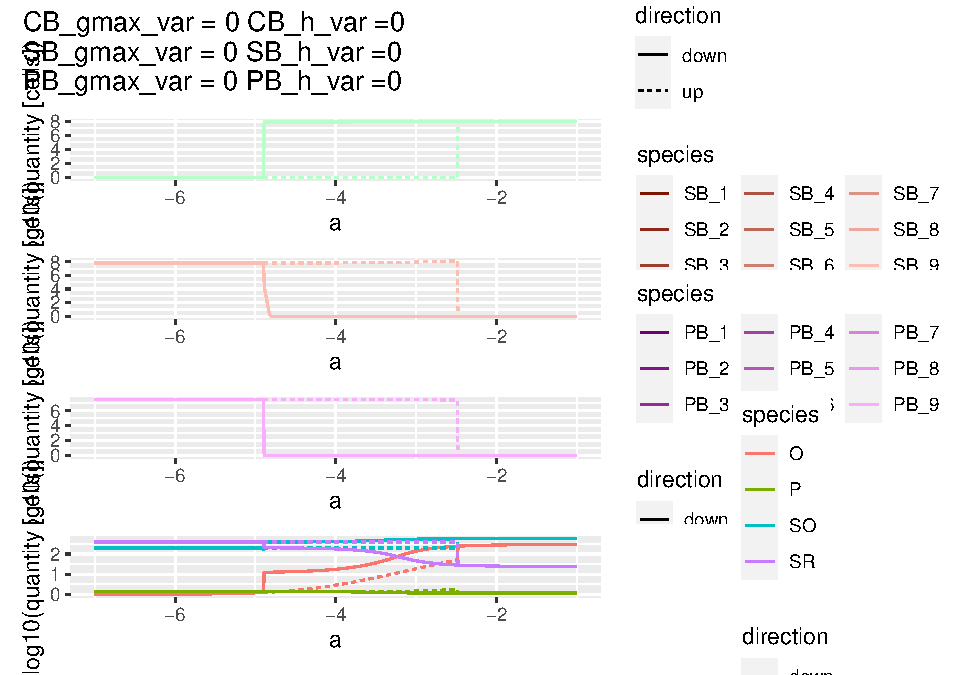
\includegraphics[width=1\linewidth]{article_files/figure-latex/ss_novar-1} 

}

\caption{your caption}\label{fig:ss_novar}
\end{figure}

X-axis must be labelled log10(a).

\hypertarget{figure-stable-states-with-variation-and-tradeoff}{%
\subsection{Figure: Stable states with variation and
tradeoff}\label{figure-stable-states-with-variation-and-tradeoff}}

\begin{figure}

{\centering 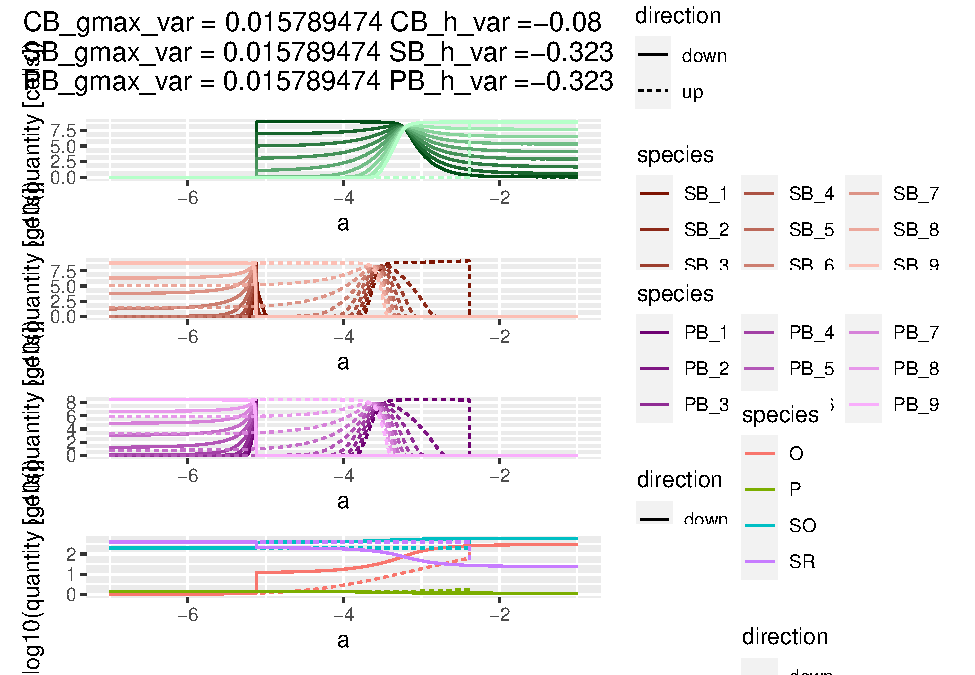
\includegraphics[width=1\linewidth]{article_files/figure-latex/ss_var-1} 

}

\caption{your caption}\label{fig:ss_var}
\end{figure}

X-axis must be labelled log10(a).

\begin{figure}

{\centering \includegraphics[width=1\linewidth]{article_files/figure-latex/ss_var2-1} 

}

\caption{your caption}\label{fig:ss_var2}
\end{figure}

X-axis must be labelled log10(a).

\hypertarget{figure-hysteresis-shift-point-nonlinearity-as-var-increases.}{%
\subsection{Figure: hysteresis, shift point, nonlinearity, as var
increases.}\label{figure-hysteresis-shift-point-nonlinearity-as-var-increases.}}

Resolution of a\_grid with 100 steps is about 0.03 units, which is about
the resolution of the y axis here. Hysteresis range is measures in
log10(a) units.

\begin{figure}

{\centering \includegraphics[width=1\linewidth]{article_files/figure-latex/ss_var3-1} 

}

\caption{your caption}\label{fig:ss_var3}
\end{figure}

\hypertarget{figure-temporal-switches}{%
\subsection{Figure: Temporal switches}\label{figure-temporal-switches}}

To be added. Need to go both ways (oxic to anoxic, and anoxic to oxic).

\hypertarget{discussion}{%
\section{Discussion}\label{discussion}}

One reason why the explanations of Dakos et al are often indeterminate
is that trait distributions can be affected by, and effect, organismal
abundances and environmental conditions. These numerous resulting
feedbacks may limit the determinancy of explanations based on the
verbal/graphical argumentation employed by Dakos et al. (2019). They may
also make for context dependent effects of functional diversity. I.e.
functional diversity may delay a tipping point in one context
(e.g.~ecosystem type and/or particular parameterisation of a specific
system) but delay it in another. \textbf{Based on our findings, (1) can
we make determinate predictions, and (2) what level of generality do our
preditions have?} {[}Possible text: The answers are (1) no, we cannot
make determinate predictions: we found sign varying effects of
functional trait diversity on the nature of ecosystem responses to
environmental change. And (2) our predictions have very limited
generality. This is because we did not aim for general predictions: we
investigate a single parameterisation of a single model, with many
explicit and implicit assumptions. This is why we need more
investigations, both theoretical and empirical, of effects of functional
trait diversity on environmental responses to environmental change.{]}

What of the empirical evidence? Hillebrand\ldots{}

What are the priorities for follow-on modelling studies?

\begin{enumerate}
\def\labelenumi{\arabic{enumi})}
\tightlist
\item
  Multifarious environmental driver changes.
\item
  More process based approach to variation in biodiversity: mutation,
  genetics,
\end{enumerate}

What does this study tell us about effects of functional diversity on
ecosystem stability?

What does this study tell us about the effects of evolution on ecosystem
stability?

\hypertarget{what-are-the-priorities-for-subsequent-research}{%
\subsection{What are the priorities for subsequent
research?}\label{what-are-the-priorities-for-subsequent-research}}

A research programme that integrates {[}text from ERC application{]}.
E.g. Global Change Microbiology -- with quote.

Then replicated across numerous ecosystems and taxa. That is, we imagine
a blue-print / template for proposals that aim to establish such an
integrative research programme. This template would contain mandatory
workpackages and experiments, and sufficient standardisation to allow
for rigorous and quantitative across programme meta-analyses

\url{https://onlinelibrary.wiley.com/doi/10.1111/gcb.15662?af=R}

\url{https://onlinelibrary.wiley.com/doi/10.1111/ele.13760?af=R}

\hypertarget{acknowledgements}{%
\section{Acknowledgements}\label{acknowledgements}}

SNF URPP

\hypertarget{bibliography}{%
\subsection*{Bibliography}\label{bibliography}}
\addcontentsline{toc}{subsection}{Bibliography}

\hypertarget{refs}{}
\begin{CSLReferences}{1}{0}
\leavevmode\hypertarget{ref-bush2017}{}%
Bush, Timothy, Muhe Diao, Rosalind J. Allen, Ruben Sinnige, Gerard
Muyzer, and Jef Huisman. 2017. {``Oxic-Anoxic Regime Shifts Mediated by
Feedbacks Between Biogeochemical Processes and Microbial Community
Dynamics.''} \emph{Nature Communications} 8 (1): 789.
\url{https://doi.org/10.1038/s41467-017-00912-x}.

\leavevmode\hypertarget{ref-ceulemans2021}{}%
Ceulemans, Ruben, Laurie Anne Wojcik, and Ursula Gaedke. 2021.
{``Functional Diversity Alters the Effects of a Pulse Perturbation on
the Dynamics of Tritrophic Food Webs.''} \emph{bioRxiv}, March,
2021.03.22.436420. \url{https://doi.org/10.1101/2021.03.22.436420}.

\leavevmode\hypertarget{ref-dakos2019b}{}%
Dakos, Vasilis, Blake Matthews, Andrew P. Hendry, Jonathan Levine,
Nicolas Loeuille, Jon Norberg, Patrik Nosil, Marten Scheffer, and Luc De
Meester. 2019. {``Ecosystem Tipping Points in an Evolving World.''}
\emph{Nature Ecology \& Evolution} 3 (3): 355--62.
\url{https://doi.org/10.1038/s41559-019-0797-2}.

\leavevmode\hypertarget{ref-hamilton2018}{}%
Hamilton, Trinity L., Judith M. Klatt, Dirk de Beer, and Jennifer L.
Macalady. 2018. {``Cyanobacterial Photosynthesis Under Sulfidic
Conditions: Insights from the Isolate Leptolyngbya Sp. Strain
Hensonii.''} \emph{The ISME Journal} 12 (2): 568--84.
\url{https://doi.org/10.1038/ismej.2017.193}.

\leavevmode\hypertarget{ref-holling1973}{}%
Holling, C S. 1973. {``Resilience and Stability of Ecological
Systems.''} \emph{Annual Review of Ecology and Systematics} 4 (1):
1--23. \url{https://doi.org/10.1146/annurev.es.04.110173.000245}.

\leavevmode\hypertarget{ref-martuxednclemente2019}{}%
Martín-Clemente, Elena, Ignacio J. Melero-Jiménez, Elena Bañares-España,
Antonio Flores-Moya, and María J. García-Sánchez. 2019. {``Adaptation
Dynamics and Evolutionary Rescue Under Sulfide Selection in
Cyanobacteria: A Comparative Study Between {\emph{Microcystis
Aeruginosa}} and {\emph{Oscillatoria}} Sp. (Cyanobacteria).''}
\emph{Journal of Phycology} 55 (6): 1348--60.
\url{https://doi.org/10.1111/jpy.12911}.

\leavevmode\hypertarget{ref-ramel2015}{}%
Ramel, Fanny, Gael Brasseur, Laetitia Pieulle, Odile Valette, Agnès
Hirschler-Réa, Marie Laure Fardeau, and Alain Dolla. 2015. {``Growth of
the Obligate Anaerobe Desulfovibrio Vulgaris Hildenborough Under
Continuous Low Oxygen Concentration Sparging: Impact of the
Membrane-Bound Oxygen Reductases.''} \emph{PLOS ONE} 10 (4): e0123455.
\url{https://doi.org/10.1371/journal.pone.0123455}.

\leavevmode\hypertarget{ref-rolfe1978}{}%
Rolfe, Rial D., David J. Hentges, Benedict J. Campbell, and James T.
Barrett. 1978. {``Factors Related to the Oxygen Tolerance of Anaerobic
Bacteria.''} \emph{Applied and Environmental Microbiology} 36 (2):
306--13. \url{https://www.ncbi.nlm.nih.gov/pmc/articles/PMC291219/}.

\leavevmode\hypertarget{ref-schoeffler2019}{}%
Schoeffler, Marine, Anne-Laure Gaudin, Fanny Ramel, Odile Valette, Yann
Denis, Wagdi Ben Hania, Agnès Hirschler-Réa, and Alain Dolla. 2019.
{``Growth of an Anaerobic Sulfate-Reducing Bacterium Sustained by Oxygen
Respiratory Energy Conservation After O {\textsubscript{2}} -Driven
Experimental Evolution: O {\textsubscript{2}} -Driven Experimental
Evolution of {\emph{Desulfovibrio}}.''} \emph{Environmental
Microbiology} 21 (1): 360--73.
\url{https://doi.org/10.1111/1462-2920.14466}.

\end{CSLReferences}

\bibliographystyle{unsrt}
\bibliography{references.bib}


\end{document}
